\chapter{Experimental Setup}\label{cha:setup}

\section{The Large Hadron Collider}\label{sec:setup:lhc}

The Large Hadron Collider (LHC)~\cite{LHC} is currently the worlds largest and most powerful proton and heavy ion accelerator.
It is located at CERN (Conseil Européen pour la Recherche Nucléaire) near Geneva.

The LHC was constructed between 1998 and 2008 inside the circular, \SI{27}{\km} long tunnel
of the former Large Electron--Positron (LEP) Collider, which was shutdown in 2000.
The tunnel is located between 50 and 175 meters below ground level and crossing the France--Switzerland border.
Both protons and heavy ions can be accelerated in two beam pipes in opposite direction.
In proton--proton collisions both beams can contain up to 2808 bunches which contain $10^{11}$ protons each.
The time distance between the bunches is \SI{25}{\ns}.
To bend the proton beams 1232 superconducting dipole magnets are used, which can generate a magnetic field of up
to \SI{8.3}{\tesla}.
Additional 392 quadrupole magnets are used to focus the beams.

The beams are collided at four \emph{interaction points} (IP), where the four major experiments
ATLAS~\cite{ATLAS}, CMS~\cite{CMS}, LHCb~\cite{LHCb}, and ALICE~\cite{ALICE} are located.
ATLAS and CMS are multipurpose detectors and are used to perform a wide range of measurements and searches.
The focus of LHCb are interactions of B-hadrons.
ALICE is specialized for measurements of heavy-ion collisions.
\cref{fig:setup:accelerators} shows a schematic overview of the LHC and its experiments.
The ATLAS experiment is discussed in detail in \cref{sec:setup:atlas}.
\begin{figure}[htb]
    \centering
    \includegraphics[width=0.9\textwidth]{./figures/setup/accelerators.png}
    \caption{The CERN accelerator complex, including the LHC and its preaccelerators.
             The four main experiments (ATLAS, CMS, LHCb, ALICE) are shown as a yellow dot~\cite{ImageLHC}.}\label{fig:setup:accelerators}
\end{figure}

The number of events per second which are generated in LHC collisions for a particular process is given by
\begin{equation}
    \label{eq:lumi:def}
    N_\text{proc} = \lumi \sigma_\text{proc} \,,
\end{equation}
where $\sigma_\text{proc}$ is the cross-section for thiss process and $\lumi$ the instantaneous luminosity.
The instantaneous luminosity is a quantity of the LHC and depends only the parameters of the beams.
For bunches with a Gaussian shape distribution it can be written as~\cite{LHC}
\begin{equation}
    \label{eq:lumi:dependencies}
    \lumi = \frac{N_b^2 n_b f_\text{ref} \gamma_r}{4 \pi \epsilon_n \beta^*} F \,,
\end{equation}
where $N_b$ is the number of particles in each bunch, $n_b$ the number of bunches per beam, $f_\text{ref}$ the revolution
frequency of the particles, $\gamma_r$ the relativistic gamma factor, $\epsilon_n$ the normalized transverse beam emittance,
$\beta^*$ the beta function at the collision point, and $F$ the geometric luminosity reduction factor
due to the crossing angle of the beams at the interaction point.
The LHC is designed to collide protons with an instantaneous luminosity of up to $\lumi = \SI{e34}{\cm\squared\per\second}$
and a beam energy of up to \SI{7}{\TeV}, which results in a collision with a center-of-mass energy of
$\sqrt{s} = \SI{14}{TeV}$.
Due to the high center-of-mass energies several preaccelerators which are shown in \cref{fig:setup:accelerators}
are needed to accelerate the particles to the desired velocity.

The first data-taking period, labeled Run-1, was in 2011 and 2012 with center-of-mass energies of $7$ and
\SI{8}{\TeV}, respectively.
A total amount of \SI{28.3}{\invfb} of data was provided by the LHC~\cite{PublicLumiRun1}.
The second data-taking period, Run-2, started in 2015 and will continue until 2018 with a center-of-mass energy of \SI{13}{TeV}.
For the years 2015 and 2016 data corresponding to an integrated luminosity of $\lumi_\text{int} = \SI{42.7}{\invfb}$ were produced~\cite{PublicLumiRun2}.

\section{The ATLAS Experiment}\label{sec:setup:atlas}

The ATLAS (A Toroidal LHC ApparatuS)~\cite{ATLAS} detector is a general-purpose detector located at LHC \emph{Point 1}
about 100 meters below ground level.
It is designed to measure properties of SM particles and processes with a high precision and for the discovery of new particles
in hadron collisions at high energies.

The detector is of cylindrical shape with a length of 40 meters and a diameter of 25 meters, and weighs around 7000 metric tons.
It is forward-backward symmetric with respect to the interaction point.

\begin{figure}[htb]
    \centering
    \includegraphics[width=0.9\textwidth]{./figures/setup/atlas.jpg}
    \caption{Overview of the ATLAS detector and its subsystems~\cite{ATLAS}.}\label{fig:setup:atlas}
\end{figure}

The ATLAS detector consists of several subdetector systems, which are illustrated in \cref{fig:setup:atlas}.
The innermost system is the inner detector (ID), which is used to measure trajectories
of charged particles, whose flight path is bent by a \SI{2}{\tesla} magnetic field, generated by a superconducting solenoid.
Next are the electromagnetic (ECal) and hadronic (HCal) calorimeters, which measure energy depositions with
liquid-argon and scintillator-tile technology.
The outermost part is the muon spectrometer (MS) which measures trajectories of muons.
An additional magnet system composed of large toroid magnets which gives the ATLAS detector its distinct look is used
to bend the trajectories of the particles again.
The different subdetectors are discussed in more detail in
\cref{sub:setup:id,sub:setup:calorimeters,sub:setup:muons}.
The general resolution goals and pseudorapidity coverage of the individual subdetectors is listed in \cref{tab:setup:resolution}.

Due to the high luminosity provided by the LHC a lot of additional inelastic scattering events occur during
a bunch crossing.
Fast readout electronics are needed to select events which are relevant to analyze.
A sophisticated trigger system as discussed in \cref{sub:setup:trigger} is used to reduce the amount of events.

\begin{table}[htpb]
    \centering
    \caption{Resolution goals and pseudorapidity coverage of the subsystems of the ATLAS detector.
            Numbers for energy and transverse momentum are in GeV.
            The notation $a \oplus b = \sqrt{a^2 + b^2}$ is used.~\cite{ATLAS}}\label{tab:setup:resolution}
    {\small
    \begin{tabular}{@{}lccc@{}}
        \toprule
        Subdetector & Required Resolution & \multicolumn{2}{c}{$\eta$-coverage}   \\
                    &                     & Measurement & Trigger \\ \midrule
        Inner Detector & $\sigma_{\pt} / \pt = 0.05\,\% \pt \oplus 1\,\%$ & $\abs{\eta} < 2.5$ & \\ \cmidrule{0-3}
        Electromagnetic & \multirow{2}{*}{$\sigma_E / E = 10\,\% / \sqrt{E} \oplus 0.7\,\%$} & \multirow{2}{*}{$\abs{\eta} < 3.2$} & \multirow{2}{*}{$\abs{\eta} < 2.5$} \\
        Calorimeter & & & \\ \cmidrule{0-3}
        Hadronic Calorimeter & & & \\
        \quad barrel and end-cap & $\sigma_E / E = 50\,\% / \sqrt{E} \oplus 3\,\% $ & $\abs{\eta} < 3.2$ & $\abs{\eta} < 3.2$ \\
        \quad forward & $\sigma_E / E = 100\,\% / \sqrt{E} \oplus 10\,\% $ & $3.1 < \abs{\eta} < 4.9$ & $3.1 < \abs{\eta} < 4.9$ \\ \cmidrule{0-3}
        Muon Spectrometer & $\sigma_{\pt} / \pt = 10\,\%$ at $\pt = \SI{1}{\TeV}$ & $\abs{\eta} < 2.7$ & $\abs{\eta} < 2.4$ \\ \bottomrule
    \end{tabular}
    }
\end{table}


\subsection{Nomenclature}\label{sub:setup:nomenclature}

The ATLAS experiment uses a right-handed coordinate system where the origin is located at the nominal interaction point.
The $x$-axis points towards the center of the LHC ring and the $y$-axis points upwards.
Therefore, the $z$-axis points counterclockwise, if viewed from above, in beam direction.
The polar angle $\theta$ is defined with respect to the $z$-axis and the azimuthal angle $\phi$ is measured
in the $x$\nobreakdash--$y$ plane.

Usual variables at hadron colliders are the energy and momentum of a particle in the transverse plane, since
they are independent on the boost of the system of the colliding particles in beam direction.
The symbols $\et$ and $\pt$ are used for the scalar quantities, respectively.
A bold symbol like $\ptvec$ is used for vectorial quantities.
The rapidity of an object is defined as
\begin{equation}
    \label{eq:rapidity}
    y = \frac{1}{2} \log \left( \frac{E + p_z}{E - p_z}\right) \,,
\end{equation}
where $p_z$ is the $z$-component of the momentum of the object.
In the case of a relativistic or massless particle ($E \gg m$) the rapidity can be replaced with the pseudorapidity $\eta$,
which is defined as
\begin{equation}
    \label{eq:pseudorapidity}
    \eta = - \log \tan \frac{\theta}{2} \,,
\end{equation}
which only depends on the polar angle $\theta$.
Differences of rapidity, $\Delta y$ and $\Delta \eta$, are \emph{Lorentz invariant} under boosts along the $z$-axis,
which is convenient when working with objects originating from hadron collisions.
This holds also true for the $\Delta R$ separation, a quantity which describes the angular separation of two objects
in the $\eta$\nobreakdash--$\Phi$ plane,
\begin{equation}
    \label{eq:deltar}
    \Delta R = \sqrt{{\left(\Delta\eta\right)}^2 + {\left(\Delta \Phi\right)}^2} \,.
\end{equation}

\subsection{Inner Detector}\label{sub:setup:id}

The ATLAS inner detector is used to measure the trajectories (tracks) and momentum of charged particles with
a transverse momentum above $\pt > \SI{0.5}{\GeV}$.
Those tracks can be used to reconstruct the primary and secondary vertices.
The ID has a cylindrical shape with a length of \SI{6.2}{\m} and diameter of \SI{2.1}{\m}.
A \SI{2}{\tesla} strong magnetic field produced by the central solenoid magnet, which cover the ID, is used to bend the flight path of the particles.
The inner detector consists of several subsystems: the pixel detector, semiconductor tracker (SCT), and transition
radiation tracker (TRT), as shown in \cref{fig:setup:id}.
Due to the close proximity of the inner detector to the beam pipe and the interaction point, the detector material
is exposed to huge amounts of radiation and high temperatures.
Therefore, extra radiation-hard material is used for the detectors.
Additionally, the pixel detector and SCT are cooled down to around \SI{-7}{\degreeCelsius} to mitigate damages.

\begin{figure}[htb]
    \centering
    \includegraphics[width=0.9\textwidth]{./figures/setup/inner_detector.jpg}
    \caption{Schematic overview of the inner detector with its submodules, the pixel detector, SCT, and TRT~\cite{ATLAS}.}\label{fig:setup:id}
\end{figure}

The pixel detector is closest to the beam pipe.
It is composed of four barrel layers and two end-caps with each three discs.
Both the barrel and end-cap layers are made of small silicon semiconductors called pixels.
The layers are segmented in $R$\nobreakdash--$\phi$ and $z$.
The innermost barrel layer is the insertable B-layer (IBL), which was only added during the shutdown period
between Run-1 and Run-2~\cite{ATLAS-TDR-19}.
The pixel detector covers the region of $\abs{\eta} < 2.5$ and reaches a hit resolution of \SI{10}{\um} in
$R$\nobreakdash--$\phi$ and \SI{115}{\um} in $z$-direction.

The semiconductor tracker uses similar concepts as the pixel detector, silicon semiconductors are used as well.
However, the used semiconductors are larger and have a strip-like geometry, which results in a worse resolution
but a larger area which is covered compared to the pixel detector.
The SCT is build out of four double layers of silicon strip detectors in the barrel part and nine layers in each of the
end-caps.
This ensures that every charged particles traverses at least four layers of detectors.
For each double layer in the barrel region one set of the silicon strip modules is aligned to the beam axis and the other set
is rotated by \SI{40}{\milli\rad}, which enables to measure the position along the beam axis.
A hit resolution of \SI{17}{\um} in the $R$\nobreakdash--$\phi$ plane and \SI{580}{\um} along the
$z$-axis is achieved which a coverage of $\abs{\eta} < 2.5$.

The outermost part of the inner detector is the transition radiation tracker.
It is made of gas-filled tubes, which are stabilized by carbon fibers.
In the barrel region the tubes are aligned to the $z$-axis, for the end-caps they are positioned radially.
Thus, only a position measurement in $R$\nobreakdash--$\phi$ in the barrel region is possible, with a
nominal hit resolution of \SI{130}{\um}.
The coverage is only $\abs{\eta} < 2.5$.
However, the TRT contributes substantially to the measurement of tracks, because of the high number of
measured points per track (usually 36 points).
Additionally, the TRT can be used for particle identification, since the transition radiation has
an inverse dependence of the mass of the charged particle.
Thus, the transition radiation is largest for electrons, which allows a discrimination from other particles.


\subsection{Calorimeters}\label{sub:setup:calorimeters}

The ATLAS calorimeter system is placed around the solenoid which produces the magnetic field inside the ID\@.
There are two types of calorimeters, the electromagnetic calorimeters and the hadronic calorimeter,
as shown in \cref{fig:setup:calo}.
They cover the full $\phi$ range and a pseudorapidity of up to $\abs{\eta} < 4.9$.
Electrons and photons are absorbed in the electromagnetic calorimeter, which enables a measurement of their energy.
The hadronic calorimter is used to determine the energy of hadrons.
The missing transverse energy as defined in \cref{eq:met:vector} is reconstructed by combining information from the two
calorimeters, the tracking detectors, and the muon spectrometer.

\begin{figure}[htb]
    \centering
    \includegraphics[width=0.9\textwidth]{./figures/setup/calorimeters.jpg}
    \caption{Schematic overview of the electromagnetic and hadronic calorimeter~\cite{ATLAS}.}\label{fig:setup:calo}
\end{figure}

Both calorimeters are \emph{sampling calorimeters}, which means that they are made of
alternating layers of active and absorbing material.
It is essential for the calorimeters that a \emph{punch-through} into the muon system is prevented.
The calorimeters has to be thick enough that all energy depositions are contained within the calorimeters.
This is important for a correct energy and \etmiss{} measurement.

\subsubsection{Electromagnetic Calorimeter}\label{subsub:setup:ecal}

The electromagnetic calorimeter is divided into the barrel region which covers $\abs{\eta} < 1.475$ and the
end-cap region within $1.375 < \abs{\eta} < 3.2$, as can be seen in \cref{fig:setup:calo}.
It uses liquid argon (LAr) as the active sampling material and lead as absorber material.

The barrel part is composed of three layers of modules.
The first layer has a fine segmentation in $\eta$ which allows a precision measurement of the position
of electrons and photons.
The second and third layer have a coarser structure and are used to collect the bulk and tail of
the electromagnetic showers, respectively.
In all layers the calorimeter modules are arranged into an accordion-shaped structure to avoid gaps
and enable coverage over the full $\phi$ range.
The energy resolution in the barrel is shown in \cref{fig:setup:calo:eres}.

The two end-caps use the same accordion geometry.
They are composed of an outer and inner wheel which cover $1.375 < \abs{\eta} < 2.5$ and $2.5 < \abs{\eta} < 3.2$, respectively.
The inner wheel is made of three layers of modules, for the outer wheel only two layers are used.

To correct for energy which is lost due to the ID and solenoid a thin LAr sampling layer called the presampler is installed
in front of the first layer in the region $\abs{\eta} < 1.8$.
For charged particles the track information of the ID can be matched to calorimeter cells within $\abs{\eta} < 2.5$ to improve
the measurement precision.

\subsubsection{Hadronic Calorimeter}\label{subsub:setup:hcal}

The hadronic calorimeter consists of three parts as shown in \cref{fig:setup:calo}.
It has a worse granularity and energy resolution than the electromagnetic calorimeter.

The tile calorimeter envelopes the electromagnetic barrel with a coverage of $\abs{\eta} < 1.0$.
It is supplemented by the two extended barrels which cover a range of $0.8 < \abs{\eta} < 1.7$.
Scintillator tiles are used as active material and steel plates as absorber.

The end-cap calorimeter consists of two wheels on each side which are used to cover the region of $1.5 < \abs{\eta} < 3.2$.
Here LAr is used as an active material and copper as an absorber.
A distribution of the energy resolution in the hadronic end-cap calorimeter is shown in \cref{fig:setup:calo:eres}.

Compared to the other two parts of the hadronic calorimeter the forward detector can also be used to reconstruct photons
and electrons, because different absorber materials are used.
In the fist module copper is used as the absorber material, whereas the second and third layer use tungsten.

The first module is used to measure electromagnetic showers with copper as the absorber.
The second and third module instead use tungsten as the absorber material which allows the measurement of hadronic showers.
All modules uses LAr as the active material.
The forward calorimeter covers a range of $3.1 < \abs{\eta} < 4.9$.

\begin{figure}[htb]
    \centering
    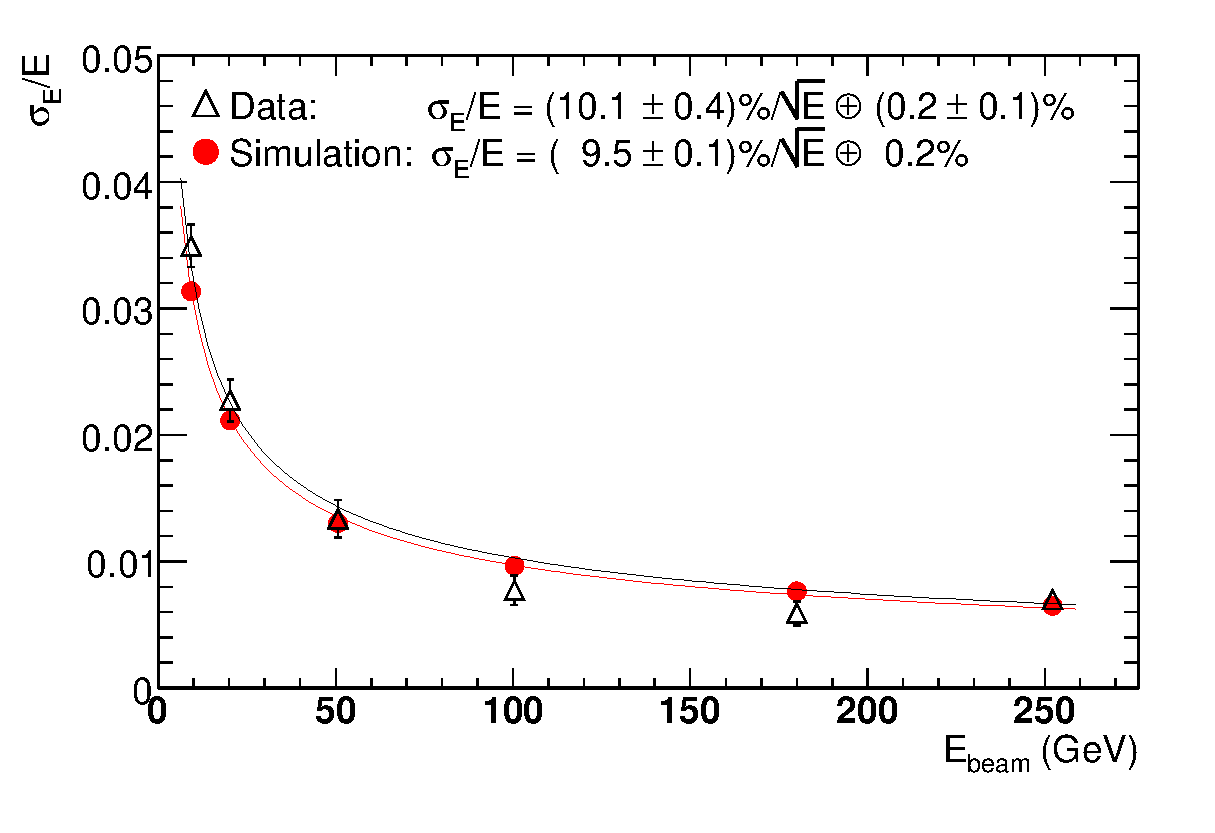
\includegraphics[width=0.45\textwidth]{./figures/setup/eres_ecal_barrel.eps}
    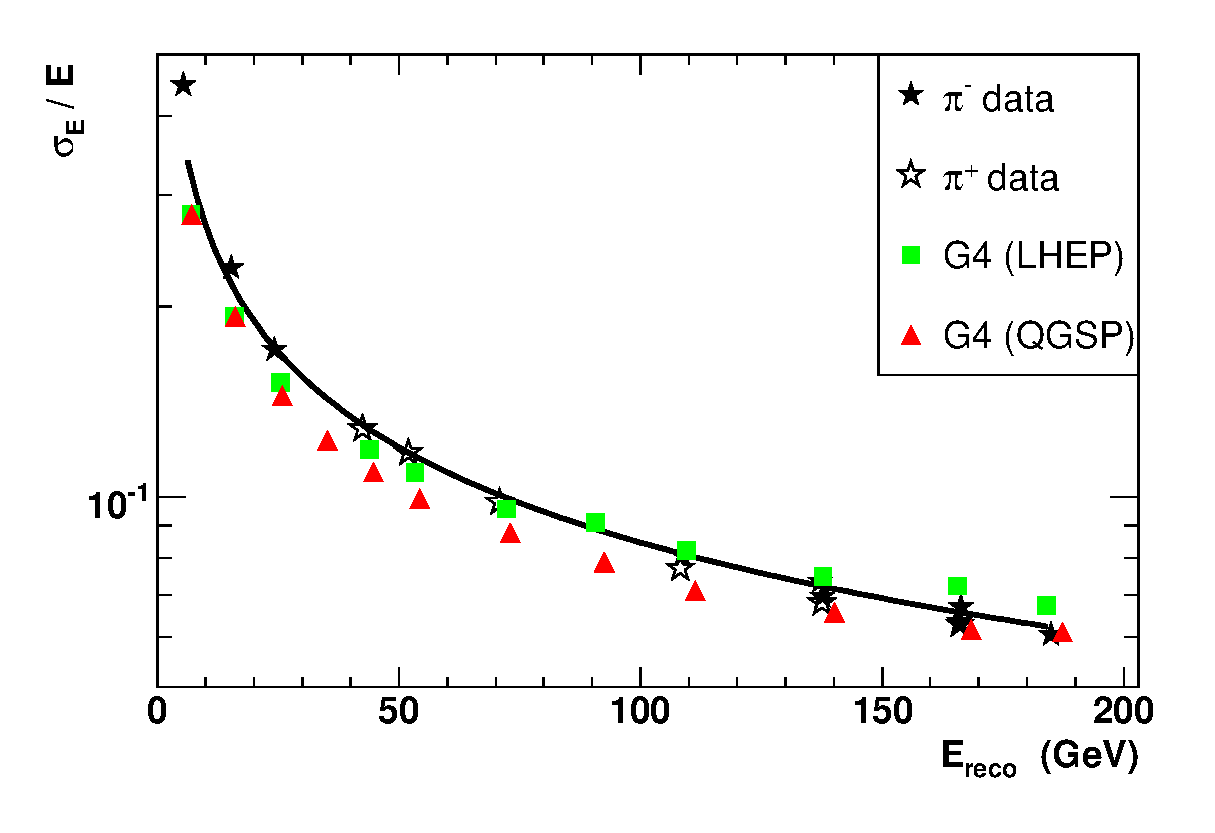
\includegraphics[width=0.45\textwidth]{./figures/setup/eres_hcal.eps}
    \caption{Comparison between test-beam measurements and simulation of the energy resolution
            in the electromagnetic barrel calorimeter (left) and for pions in the
            hadronic end-cap calorimeter (right)~\cite{ATLAS}.}\label{fig:setup:calo:eres}
\end{figure}


\subsection{Muon Spectrometer}\label{sub:setup:muons}

The muon spectrometer is used to detect charged particles which pass the electromagnetic and hadronic calorimeters.
These particles are mainly muons, since all other particles should deposit all their energy in the calorimeters.
The MS is the outermost part of the ATLAS detector.
A schematic overview can be found in \cref{fig:setup:muon}.
It is composed of three regions: the barrel region covering $\abs{\eta} < 1.4$, the end-cap region which covers $1.6 < \abs{\eta} < 2.7$,
and the transition region, which covers the region $1.4 < \abs{\eta} < 1.6$ between the two aforementioned regions.
In the barrel region three layers of muon chambers are used, whereas four wheels perpendicular to the beam axis are installed
in the end-cap region.

Large toroidal magnets produce the magnetic field needed for the momentum measurements.
There are two different magnet systems, one for the barrel part and one for the end-caps, with strengths up to
\SI{2.5}{\tesla} and \SI{3.5}{\tesla}, respectively.
In the transition region the magnetic fields of both systems are used.
In total 24 coils are used.

\begin{figure}[htb]
    \centering
    \includegraphics[width=0.9\textwidth]{./figures/setup/muon.jpg}
    \caption{Schematic overview of the ATLAS muon spectrometer with its different regions and the toroid system~\cite{ATLAS}.}\label{fig:setup:muon}
\end{figure}

In most parts of the MS the trajectories of the muons are measured by monitored drift tubes,  which provide a resolution
of \SI{35}{\um} per chamber.
The one exception is the range of $2.0 < \abs{\eta} < 2.7$ in the forward region, where cathode strip-chambers are used
in the innermost layer.
They provide a higher rate capability and time resolution.
However, a spatial resolution of only \SI{40}{\um} in the bending plane and \SI{5}{\mm} in the
transverse plane is achieved.

The muon system also provides a trigger for particles in the range $\abs{\eta} < 2.4$.
Resistive plate chambers are used in the barrel region and thin gap chambers in the end-cap region, which
achieve a response time of a few nanoseconds.

\subsection{Trigger System}\label{sub:setup:trigger}

Particle bunches at the LHC have a time separation of \SI{25}{\ns}, therefore the rate of collisions is \SI{40}{\MHz}.
However, only a small amount of the collision events can be recorded and further analyzed, due to the huge amount of data which is produced.
A two level trigger-system is used to select events which are relevant for physics analyses.
It is composed of the hardware-based first level trigger (L1) and the software-based high level trigger (HLT).
An schematic overview is given in \cref{fig:setup:trigger}.

\begin{figure}[htb]
    \centering
    \includegraphics[width=0.9\textwidth]{./figures/setup/trigger.pdf}
    \caption{The ATLAS trigger and data acquisition system for Run-2.\cite{ImageTrigger}}\label{fig:setup:trigger}
\end{figure}

The hardware-based L1 trigger uses coarse granularity information of calorimeters and the muon chambers provided by custom hardware
to detect events where particles like electrons, $\tau$-leptons, and jets have a high transverse energy.
Events with large missing transverse energy or where muons have a large transverse momentum are also triggered.
The decision time to accept an event is \SI{2.5}{\us} and results in an event rate of \SI{100}{\kHz}.
Furthermore, the L1 trigger sends the $\eta$ and $\phi$ coordinates which caused the L1 trigger to fire,
the so called \emph{region of interest} (ROI), to the HLT\@.

The high level trigger uses information in the ROI at full granularity.
It reduced the event rate to around \SI{1}{\kHz} with a decision time of \SI{200}{\ms}.

Several triggers are provided in a \emph{trigger menu} based on the number of objects,
amount of transverse momentum or missing transverse energy, and certain identification and
isolation criteria.
\cref{fig:setup:triggermenu} shows different triggers and their rates for data taken in July 2016.
The triggers which are used in this analysis are discussed in detail in \cref{sec:event_selection:trigger}.

\begin{figure}[htb]
    \centering
    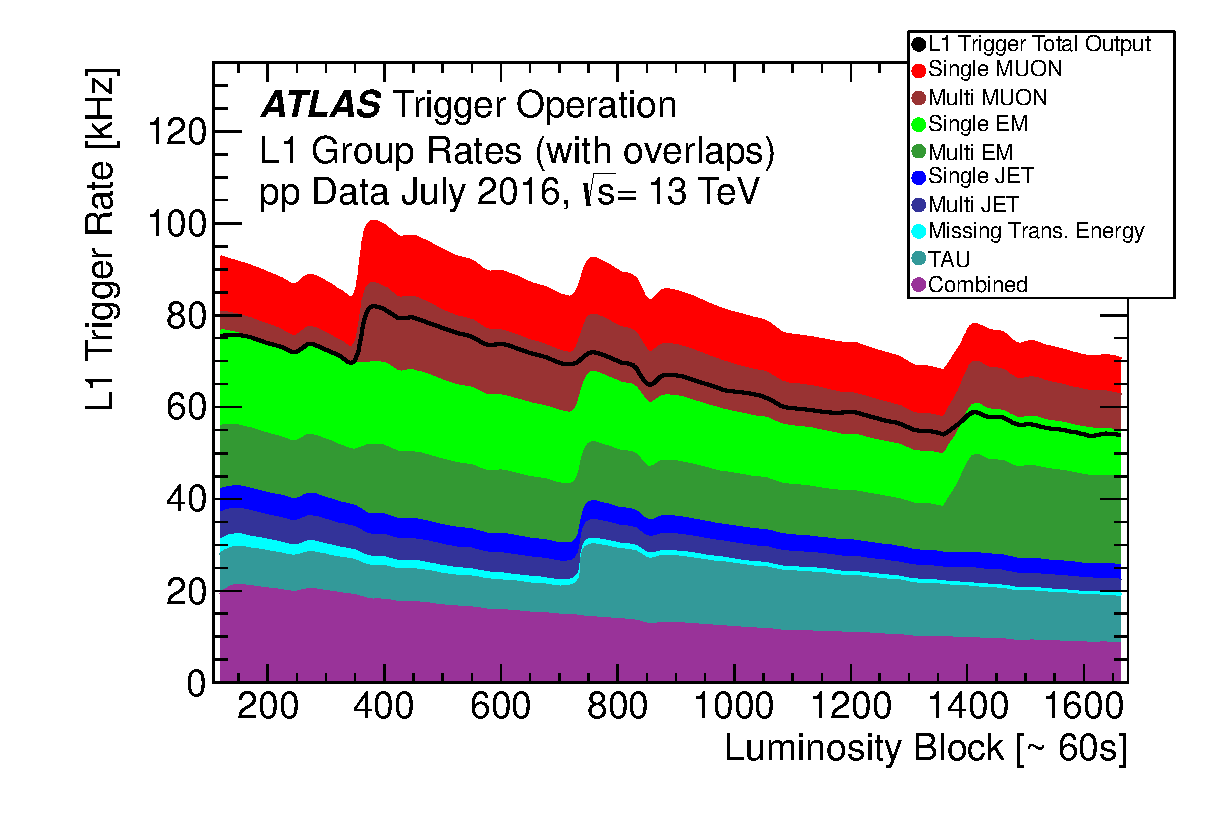
\includegraphics[width=0.45\textwidth]{./figures/setup/l1_trigger_menu_2016.eps}
    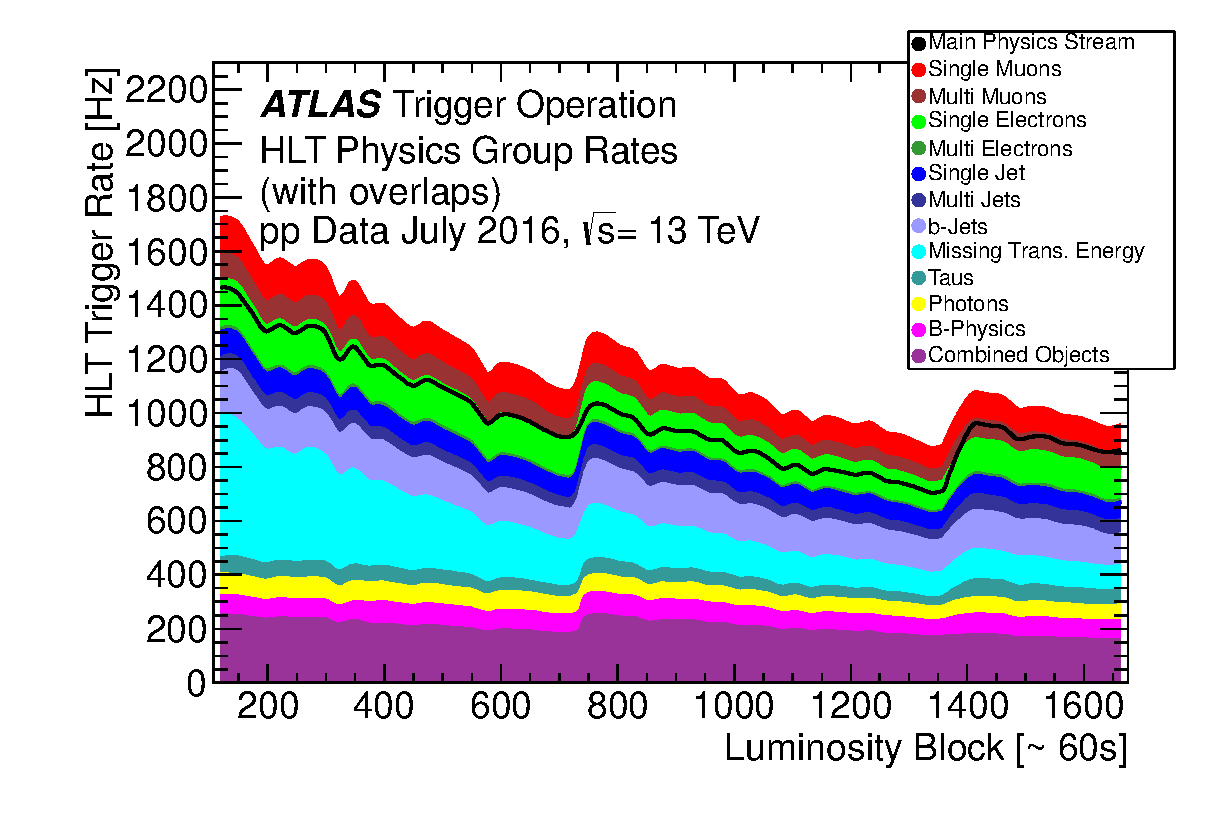
\includegraphics[width=0.45\textwidth]{./figures/setup/hlt_trigger_menu_2016.eps}
    \caption{Trigger menu and rates for the L1 trigger (left) and HLT (right) for data taken in July 2016~\cite{TriggerMenu2016}.}\label{fig:setup:triggermenu}
\end{figure}


\subsection{Data taking in 2015 and 2016}\label{sec:setup:data}

During 2015 and 2016 the ATLAS experiment recorded data from proton--proton collisions at a center-of-mass energy
of $\sqrt{s} = \SI{13}{\TeV}$, which corresponds to an integrated luminosity of \SI{3.9}{\invfb} and \SI{35.6}{\invfb}, respectively.
Not all data satisfies imposed data quality criteria, which are discussed in \cref{sec:event_selection:preselection},
therefore not all data can be used for physics analyses.
This analysis uses data corresponding to \SI{3.21}{\invfb} and \SI{32.86}{\invfb} for 2015 and 2016, respectively.
The uncertainty on the luminosity measurement is \SI{2.1}{\percent}~\cite{LumiUncertRun2}.

Because there are $10^{11}$ protons in each bunch it is likely that more than one interaction occurs per bunch crossing.
This is called \emph{in-time pile-up}.
Due to the low time distance of \SI{25}{\ns} between each bunch crossing interactions which happen directly before or after
the interaction of interest can also be recorded, since the read out time of the calorimeters is much slower.
This is called \emph{out-of-time pile-up}.
The mean of total interactions per bunch crossing in data taken in 2015 and 2016 is $23.7$~\cite{PublicLumiRun2}.
\cref{fig:setup:pileup} shows a distribution of the mean pile-up for data taken in 2015 and 2016.

\begin{figure}[htb]
    \centering
    \includegraphics[width=0.4\textwidth]{./figures/setup/pileup_2015_2016.eps}
    \caption{Distribution of the mean number of interactions per bunch crossing (pile-up)
             weighted by luminosity for data taken in 2015 and 2016~\cite{PublicLumiRun2}.}\label{fig:setup:pileup}
\end{figure}
